\documentclass{beamer}
\usepackage[T1]{fontenc}

%\documentclass[aspectratio=169]{beamer}
%\usetheme{Madrid} % My favorite!
%\usetheme{Boadilla} % Pretty neat, soft color.
%\usetheme{default}
%\usetheme{Warsaw}
%\usetheme{Bergen} % This template has nagivation on the left
%\usetheme{Frankfurt} % Similar to the default 
%\usetheme{Copenhagen}
\usetheme{Goettingen}
%with an extra region at the top.
\usecolortheme{seahorse} % Simple and clean template
%\usetheme{Darmstadt} % not so good
% Uncomment the following line if you want %
% page numbers and using Warsaw theme%
% \setbeamertemplate{footline}[page number]
%\setbeamercovered{transparent}
\setbeamercovered{invisible}
\setbeamersize{text margin right=3.5mm, text margin left=7.5mm}  % text margin
\setbeamertemplate{caption}[numbered]

\setbeamerfont{page number in head/foot}{size=\large}
\setbeamertemplate{footline}[frame number]


% To remove the navigation symbols from 
% the bottom of slides%
%
\usepackage{graphicx}

\usepackage[
backend=biber,
autocite=superscript,
natbib=true,
style=numeric,
sorting=none]{biblatex}

\addbibresource{TrustCom15.bib}
\usepackage{tikz}
\usepackage{calc}


\usepackage{amsmath,amsthm, amssymb, latexsym}
\usepackage{booktabs}
\usepackage{colortbl}
\usepackage{hyperref}
%\usepackage[textsize=tiny]{todonotes}
%\presetkeys{todonotes}{inline}{}

\interdisplaylinepenalty=2500
\hyphenpenalty=10000

\usepackage[caption=false,font=scriptsize,justification=centerlast]{subfig}
\usepackage[english]{babel}
\addto\captionsenglish{\renewcommand{\figurename}{Fig.}}

\def\checkmark{\tikz\fill[scale=0.4](0,.35) -- (.25,0) -- (1,.7) -- (.25,.15) -- cycle;} 
\def\scalecheck{\resizebox{\widthof{\checkmark}*\ratio{\widthof{x}}{\widthof{\normalsize x}}}{!}{\checkmark}}
%that's defined it - now for a test

\makeatletter
\newcommand*{\minuscellcolor}{}
\def\minuscellcolor\ignorespaces{%
	% \ignorespaces not really needed, because \@ifnextchar gobbles spaces
	
	\@ifnextchar-{\cellcolor[HTML]{FFAAAA}}{}
}
\newcolumntype{L}{>{\minuscellcolor}l}
\newcolumntype{C}{>{\minuscellcolor}c}
\newcolumntype{R}{>{\minuscellcolor}r}
\makeatother

\graphicspath{{../Figures/}{../posters/PDW-15/figures/},{./img/}}
\DeclareGraphicsExtensions{.pdf,.png,.jpg}
%\usepackage{bm}         % For typesetting bold math (not \mathbold)
%\logo{\includegraphics[height=0.6cm]{yourlogo.eps}}
%

\title[Multi-Metric Trust in UANs]{Single and Multi-Metric Trust Management Frameworks for use in Underwater Autonomous Networks}

\author[Bolster, A \& Marshall A]{Andrew Bolster and Alan Marshall}
\institute[UoL]
{
University of Liverpool \\
\medskip
{\emph{\{andrew.bolster,alan.marshall\}@liv.ac.uk}}\\
\vspace{0.3in}

\includegraphics[width=0.5\textwidth]{img/livuni}%
}
\date[TrustCom RATSP 2015]{Recent Advances of Trust, Security and Privacy in Computing Communications (RATSP)}
% \today will show current date. 
% Alternatively, you can specify a date.
%

% If you have a file called "university-logo-filename.xxx", where xxx
% is a graphic format that can be processed by latex or pdflatex,
% resp., then you can add a logo as follows:

% \pgfdeclareimage[height=0.5cm]{university-logo}{university-logo-filename}
% \logo{\pgfuseimage{university-logo}}



% Delete this, if you do not want the table of contents to pop up at
% the beginning of each subsection:
\AtBeginSubsection[]
{
  \begin{frame}<beamer>{Outline}
    \tableofcontents[currentsection,currentsubsection]
  \end{frame}
}


\begin{document}

\begin{frame}
  \titlepage
\end{frame}

\frame{\tableofcontents}
%

\section{Motivation}


\begin{frame}{Summary}
  % - A title should summarize the slide in an understandable fashion
  %   for anyone how does not follow everything on the slide itself.

  \begin{itemize}
  \item
    Trust Methods in the MANET space applied to other arenas (e.g. underwater acoustics).
  \item
    Trust Management Frameworks (TMFs) require reassessment to work in the harsh marine communications environment.
  \item 
    Most rely on one type of observation (metric)
  \item 
    Recent work\autocite{Guo11} introduces the use of multiple types of continuous metrics for assessment.
    \pause
  \item 
    How do these Single and Multi-Metric Frameworks perform in the challenging marine communications environment?
  \item
    What metrics are suitable for use underwater?
  \end{itemize}
\end{frame}



\subsection{Related Work}

\begin{frame}{Trust in Conventional MANETS}
  \begin{itemize}
    \item 
      TMFs provide information to assist the estimation of future states and actions of nodes within networks.
      \pause
    \item
      Centralised methods unsuitable for dynamic networks in terms of efficiency and robustness\autocite{Caiti2011}.
      \pause
    \item 
      Need to detect, identify, \& mitigate threats in a distributed fashion.
  \end{itemize}
\end{frame}

\begin{frame}[allowframebreaks]{Single-Metric TMFs}
  Most can be generalised as single-value estimations of PLR/Successful Routes, with the incorporation of some \emph{meta}-observations e.g. Topology
  \begin{itemize}
    \item \emph{Hermes} \autocite{Zouridaki2005} - Bayesian estimation based on PLR
    \item \emph{OTMF} \autocite{Li2008} - Collaborative Bayesian Trust
    \item \emph{TSR} \autocite{Moe2008a} - HMM route assessment, Session Loss Rate.
    \item \emph{CONFIDANT} \autocite{Buchegger2002} - Probabilistic PLR assessment, includes topology and reputation weighting.
    \item \emph{Fuzzy Trust-Based Filtering} \autocite{Luo2008} - Fuzzy classification of packet delivery
  \end{itemize}
  \framebreak
  \begin{itemize}
  \item
    Opportunities for malicious actors to undermine the operation of a network. 
  \item 
    Not an issue in networks where Comms. is the primary operating concern, but is significant in resource constrained environments
  \end{itemize}

\end{frame}

\begin{frame}{Multi-Metric TMF} 
  \emph{Multi-metric Trust For MANETS (MTFM)} \autocite{Guo11} 
  \begin{itemize}
    \item Additional metrics as well as PLR, 
    \item Topological relationship,
    \item Metric weighting enables behaviour classification
    \item Grey Relational Grading provides dynamic runtime normalisation, assessing \emph{comparative} trust within a cohort of actors.
  \end{itemize}
  \pause
  \centering
  Operates favourably in 802.11 against OTMF and Hermes, accurately detecting, identifying, \& characterising misbehaviours.\autocite{Guo11} 
\end{frame}
\begin{frame}{Multi-Metric TMF - Grey Grading} 
\begin{equation}
  \label{eq:grcg}
  \theta_{k,j}^t = \frac{\min_k|a_{k,j}^t - g_j^t| + \rho \max_k|a_{k,j}^t-g_j^t|}{|a_{k,j}^t-g_j^t| + \rho \max_k|a_{k,j}^t-g_j^t|} 
\end{equation}
\begin{equation}
  \label{eq:grcb}
  \phi_{k,j}^t = \frac{\min_k|a_{k,j}^t - b_j^t| + \rho \max_k|a_{k,j}^t-b_j^t|}{|a_{k,j}^t-b_j^t| + \rho \max_k|a_{k,j}^t-b_j^t|} 
\end{equation}
\begin{equation}
  \label{eq:grc}
  [\theta_k^t, \phi_k^t] = \left[\sum_{j=0}^M h_j \theta_{k,j}^t,\sum_{j=0}^M h_j \phi_{k,j}^t \right]
\end{equation}
\begin{equation}
  \label{eq:grcT}
  T_k^t = ({1+{(\phi_k^t)^2}/{(\theta_k^t)^2}})^{-1}
\end{equation}

Where  $a_{k,j}^t$ is the value of an observed metric $x_j$ for a given node $k$ at time $t$,  $g$ and $b$ are respectively the ``good'' and ``bad'' reference metric sequences from $\{a_{k,j}^t k=1,2\dots K\}$, $H=[h_0\dots h_M]$ is a metric weighting vector such that $\sum h_j = 1$

\end{frame}
\begin{frame}{Multi-Metric TMF - Topological Relationships} 
  \centering
  Includes shared assessments from other nodes weighted based on their relative topology to provide a final value\footnotemark  

  \vspace{9pt}

  $T_{i,j}^{MTFM}$
    \begin{figure}[h]
      \centering
      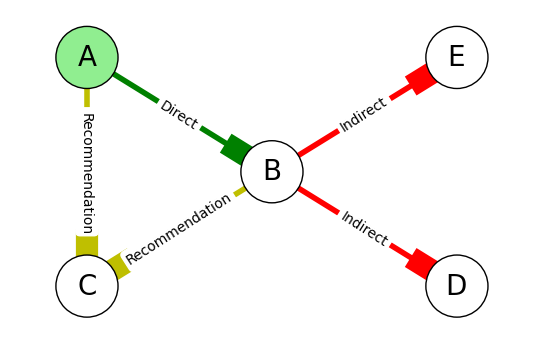
\includegraphics[width=.9\textwidth]{node_relationships}
      \label{fig:node_relationships}
    \end{figure}
    \footnotetext{\hyperlink{eq:networkeffects}{\beamergotobutton{Details}}}

\end{frame}

\subsection{Challenges to Trust in Underwater Networks}

\begin{frame}{Communications Channel Considerations}
  Key Characteristics of the Marine Acoustic Channel \autocite{Urick1983a,Partan2006,Stojanovic2007,Stefanov2011}:
  \begin{itemize}
    \item Slow propagation ($~1400ms^{-1}$) incurring long delays
    \item Inter-symbol interference
    \item Doppler Spreading
    \item Non-Linear propagation due to refraction
    \item Fast \& Slow fades from environmental factors (flora/fauna/surface and seabed conditions)
    \item Freq. dependant attenuation
    \item Significant destructive multipath effects
  \end{itemize}
  
\end{frame}

\begin{frame}{Attenuation in the Marine Acoustic Channel}

  The attenuation that occurs in an underwater acoustic channel over distance $d$ about frequency $f$ is given as $A_{\text{aco}}(d,f) = A_0d^ka(f)^d$ or
  %
  \begin{equation}
    \label{eq:acoattenuationdb}
    10 \log A_{\text{aco}}(d,f)/A_0 = k \cdot 10 \log d + d \cdot 10 \log a(f)
  \end{equation}
  %
  where $A_0$ is a normalising constant, $k$ is a spreading factor, and $a(f)$ is the absorption coefficient\autocite{Stefanov2011};
  %
  \begin{equation}
    \label{eq:thorp}
    10 \log a(f) = \frac{0.11 \cdot f^2}{1+f^2} + \frac{44\cdot f^2}{4100+f^2}+ 2.75\times10^{-4} f^2 + 0.003
  \end{equation}

  \pause

  Compared to RF Free space PL: $(A_{\text{RF}}(d,f) \approx \left( \frac{4\pi d f}{c} \right)^2)$
  \begin{itemize}
    \item \alert{Exponential} in $d$: $A_{\text{aco}} \propto f^{d}$ vs $A_{\text{RF}} \propto (df)^2$
    \item $f$ factor \alert{four orders higher} in $f\propto A_{\text{aco}}$ vs $f\propto A_{\text{RF}}$

  \end{itemize}
  
\end{frame}
\begin{frame}{Operational Considerations: Collaborative AUV Survey}
  \begin{columns}
    \begin{column}{0.5\textwidth}
      Context:
      \begin{itemize}
        \item Fleets of up to 16 collaborating Autonomous Underwater Vehicles(AUVs)
        \item Constrained in Power, Mobility, Processing, Storage Capacity
        \item Tasked to perform ongoing survey of an area
      \end{itemize}

      \uncover<2->{\centering
      Communications Efficiency is not the only factor at risk from malicious exploitation}
    \end{column}
    \begin{column}{0.5\textwidth}
      \begin{figure}[h]
        \begin{center}
          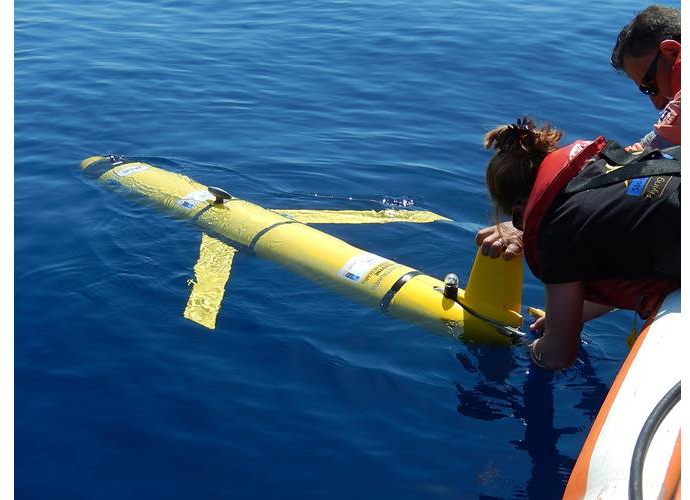
\includegraphics[width=\linewidth]{remus100cmre}
        \end{center}
        \caption{REMUS 100 AUV as deployed at NATO CMRE La Spezia}
        \label{fig:remus100cmre}
      \end{figure}
      
    \end{column}
  \end{columns}
\end{frame}



\section{Our Contribution}

\subsection{Experimental Context}

\begin{frame}{Misbehaviour Specification}
  \begin{itemize}
    \item Two misbehaviours investigated:
      \begin{itemize}
        \item \emph{Malicious Power Control}(MPC) - attacker aims to make a node appear selfish by increasing power to all nodes except to/from it
        \item \emph{Selfish Target Selection}(STS) - node preferentially communicates with nodes close to it, to conserve its own power.
      \end{itemize}
    \item Neither misbehaviour \alert{directly} affects PLR, while impacting network fairness,

    \item Default Behaviour: random walk with ``Fair'' communications

    \item Three Scenarios:
      \begin{itemize}
        \item All nodes are Fair
        \item One node is Malicious (MPC)
        \item One node is Selfish (STS)
      \end{itemize}
  \end{itemize}

\end{frame}

\begin{frame}[label=scaling]{Scaling Considerations}
  \begin{itemize}
    \item Simulations based on SimPy \autocite{Mueller2003SimPy}, Network stack using AUVNetSim \autocite{Miquel2008} and channel constraints based on Stojaovic and Stefanov \autocite{Stojanovic2007,Stefanov2011}\hyperlink{tab:sysconstraints}{\beamergotobutton{Details}}
      \pause
    \item Established a safe operating zone optimising for delay/throughput  \hyperlink{eq:networkeffects}{\beamergotobutton{Details}}
    \item Six per-link communications metrics
      \pause\begin{columns}
        \begin{column}{0.5\textwidth}
          \begin{itemize}
            \item Received Power
            \item Received Throughput
            \item E2E Delay
          \end{itemize}
        \end{column}
        \begin{column}{0.5\textwidth}
          \begin{itemize}
            \item Transmitted Power
            \item Transmitted Throughput
            \item Packet Loss Rate
          \end{itemize}
        \end{column}
      \end{columns}
  \end{itemize}

\end{frame}

\subsection{MTFM Operation}

\begin{frame}[allowframebreaks]{Multi-Metric Operation}
  \label{trust_mobility_summary}
  \setcounter{subfigure}{0}% Reset subfigure counter
  \begin{figure}[htp]
    \centering
    \subfloat[Fair Static]{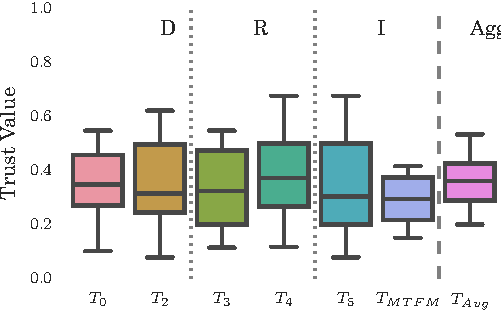
\includegraphics[width=0.33\linewidth]{trust_bella_static_fair} \label{fig:trust_static}}\hfil
    \subfloat[Malicious Static]{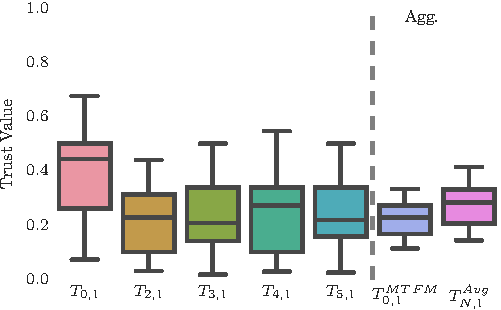
\includegraphics[width=0.33\linewidth]{trust_bella_static_malicious} \label{fig:trust_static_mal}}\hfil
    \subfloat[Selfish Static]{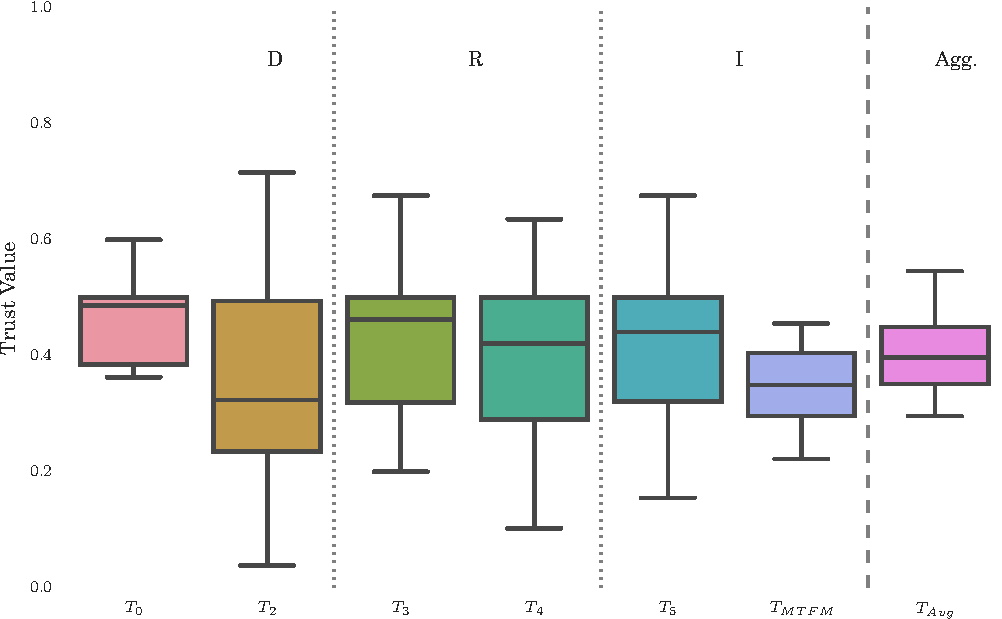
\includegraphics[width=0.33\linewidth]{trust_bella_static_selfish} \label{fig:trust_static_sel}}\hfil

    \subfloat[Fair Mobile]{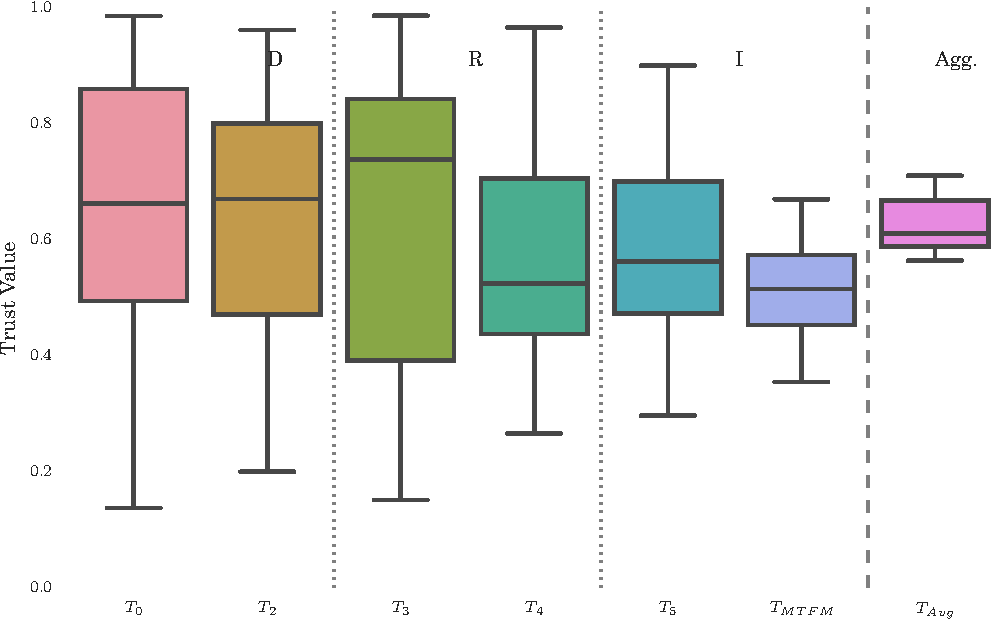
\includegraphics[width=0.33\linewidth]{trust_bella_all_mobile_fair}  \label{fig:trust_all_mobile}}\hfil
    \subfloat[Malicious Mobile]{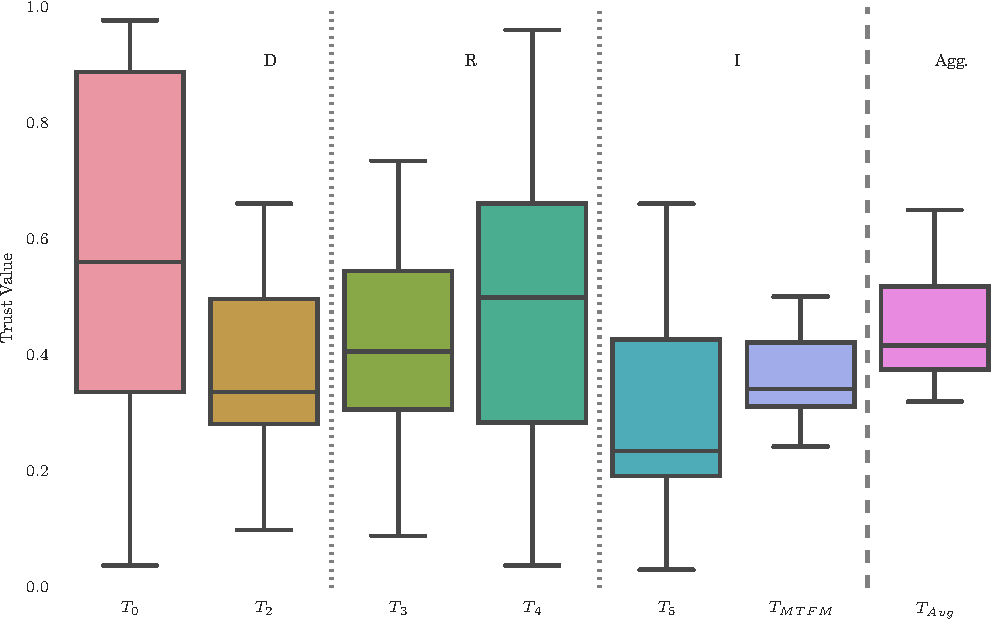
\includegraphics[width=0.33\linewidth]{trust_bella_all_mobile_malicious}  \label{fig:trust_all_mobile_mal}}\hfil
    \subfloat[Selfish Mobile]{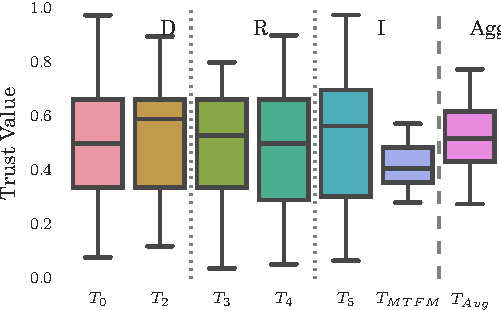
\includegraphics[width=0.33\linewidth]{trust_bella_all_mobile_selfish}  \label{fig:trust_all_mobile_sel}}\hfil
    \caption{Observations of $n_1$ ($T_{1,X}$), showing Direct, Recommender and Indirect relationships and $T_{MTFM}$ and $T_{AVG}$Y\hyperlink{fig:trust_mobility_closeup}{\beamergotobutton{Closeup}}}
    \label{fig:trust_mobility}
  \end{figure}
%\end{frame}
\framebreak
Key Observations: 
%\begin{frame}{Multi-Metric Operation - Key Observations}
  %
  \begin{itemize}
    \item Mobility greatly increases variation in observed trust
    \item $T_{MTFM}$ remains more stable in both mobility cases when compared to either single-node assessments or $T_{Avg}$
    \item Raw $T_{MTFM}$ isn't perfect; results demonstrate huge variability in Direct assessment ($T_{1,0}$) that isn't reflected in $T_{MTFM}$.
    \item Larger variability in ``Fair'' case compared to MPC/STS
  \end{itemize}
  \centering
  Considering the mobility results and stated context, we continue with mobile-only scenarios.
\end{frame}

\subsection{Single vs Multi}

\begin{frame}{Blind Comparison of Single/Multi-metric TMFs}
  \vspace{-24pt}%
  \begin{columns}
    \begin{column}[T]{0.5\textwidth}
      \begin{figure}[t]
        \centering
        \subfloat[Fair Scenario]{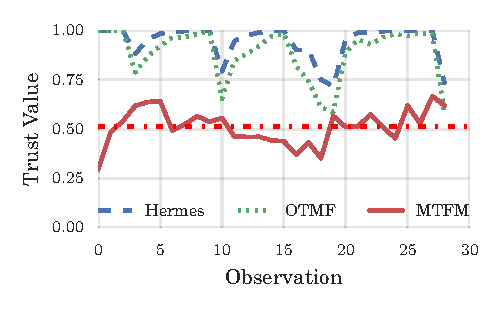
\includegraphics[width=\linewidth]{trust_beta_otmf_fair} \label{fig:all_mobile_fair_beta}}\hfil
        \renewcommand{\thesubfigure}{c}% New fixed/manual numbering
        \subfloat[Selfish Target Selection Scenario]{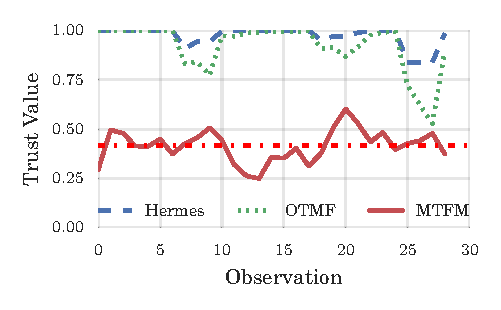
\includegraphics[width=\linewidth]{trust_beta_otmf_selfish} \label{fig:all_mobile_selfish_beta}}
        \label{fig:otmf_beta_comparison}
      \end{figure}%
    \end{column}
    \begin{column}[T]{0.5\textwidth}
      \begin{figure}[t]
        \centering
        \vspace{0pt}%
        \renewcommand{\thesubfigure}{b}% New fixed/manual numbering
        \subfloat[Malicious Power Control Scenario]{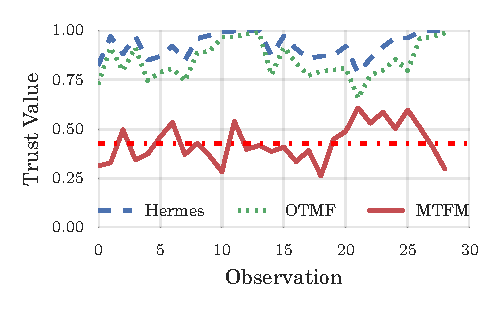
\includegraphics[width=\linewidth]{trust_beta_otmf_malicious} \label{fig:all_mobile_badmouthing_beta}}
        \label{fig:otmf_beta_comparison}
      \end{figure}
      $T_{1,0}$ for Hermes, OTMF and MTFM assessment values for fair and malicious behaviours in the fully mobile scenario (mean of MTFM also shown)

    \end{column}
  \end{columns}

  \framebreak
\end{frame}
\begin{frame}{Blind Comparison of Single/Multi-metric TMFs}

  Key Observations:
  \begin{itemize}
    \item Everybody Sucks
    \pause\item Neither OTMF, Hermes or Blind MTFM are effective
    \item MTFM's Comparison means in the fair case, $\approx0.5$ is expected
    \item In OTMF/Hermes, $T\approx1$ is expected
    \pause\item MTFM indicates $\approx10\%$ selectivity between Fair and Either Misbehaviour
  \end{itemize}
  \pause \alert{BUT!}  \pause MTFM allows exploration of the metric space.

\end{frame}

\subsection{Metric Weighting}
\begin{frame}{Metric Weighting}
  From \eqref{eq:grc}, metric emphasise can be adjusted
  \begin{align}
    [\theta_k^t, \phi_k^t]& = \left[\sum_{j=0}^M h_j \theta_{k,j}^t,\sum_{j=0}^M h_j \phi_{k,j}^t \right]\\
    T_k^t &= ({1+{(\phi_k^t)^2}/{(\theta_k^t)^2}})^{-1}
  \end{align}
\end{frame}

\begin{frame}{Malicious Power Control - Weighted Emphasis}
    \label{fig:all_mobile_badmouthing}
  \vspace{-24pt}%
\setcounter{subfigure}{0}% Reset subfigure counter
  \begin{figure}[h]
    \centering
    \subfloat[Delay Emphasised]{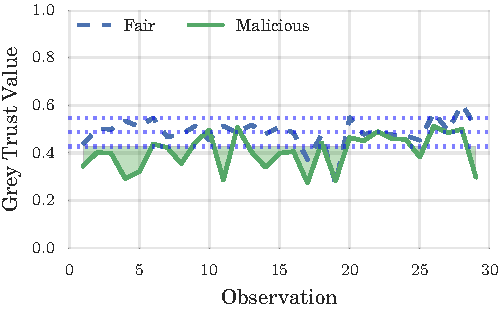
\includegraphics[width=.33\linewidth]{img/trust_bella_all_mobile_emph_ADelay_BadMouthingPowerControl} \label{fig:all_mobile_badmouthing_delay}}
    \subfloat[PLR Emphasised]{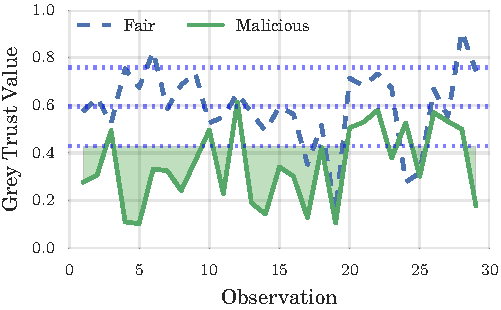
\includegraphics[width=.33\linewidth]{img/trust_bella_all_mobile_emph_PLR_BadMouthingPowerControl}\label{fig:all_mobile_badmouthing_plr}}
    \subfloat[RX Power Emphasised]{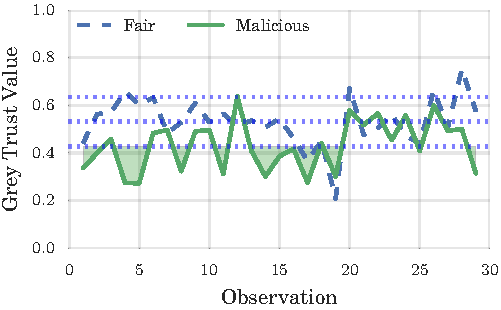
\includegraphics[width=.33\linewidth]{img/trust_bella_all_mobile_emph_ARXP_BadMouthingPowerControl} \label{fig:all_mobile_badmouthing_rxp}}
    \newline
    \subfloat[TX Power Emphasised]{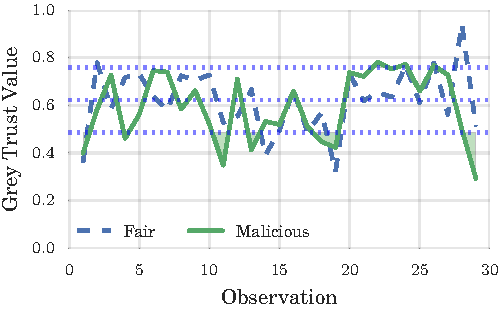
\includegraphics[width=.33\linewidth]{img/trust_bella_all_mobile_emph_ATXP_BadMouthingPowerControl}\label{fig:all_mobile_badmouthing_txp}}
    \subfloat[RX Throughput Emphasised]{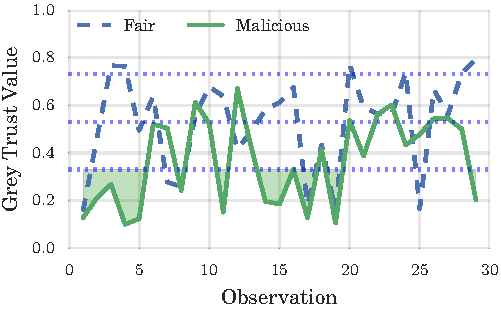
\includegraphics[width=.33\linewidth]{img/trust_bella_all_mobile_emph_RXThroughput_BadMouthingPowerControl} \label{fig:all_mobile_badmouthing_rxthroughput}}
    \subfloat[TX Throughput Emphasised]{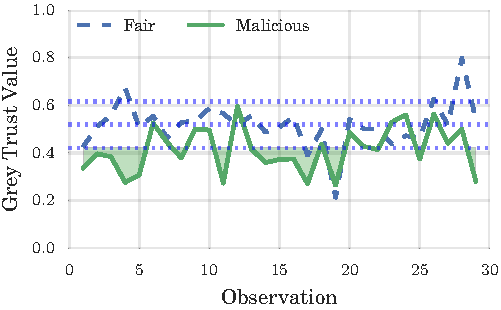
\includegraphics[width=.33\linewidth]{img/trust_bella_all_mobile_emph_TXThroughput_BadMouthingPowerControl} \label{fig:all_mobile_badmouthing_txthroughput}}
    \caption{$T_{1,MTFM}$ in the All Mobile case for the Malicious Power Control behaviour, including dashed $\pm\sigma$ envelope about the fair scenario\hyperlink{fig:badmouth_emph_closeup}{\beamergotobutton{Closeup}}}
  \end{figure}
\end{frame}

\begin{frame}{Selfish Target Selection - Weighted Emphasis}
\label{fig:all_mobile_selfish}
  \vspace{-24pt}%
\setcounter{subfigure}{0}% Reset subfigure counter
  \begin{figure}[h]
  \centering
  \subfloat[Delay Emphasised]{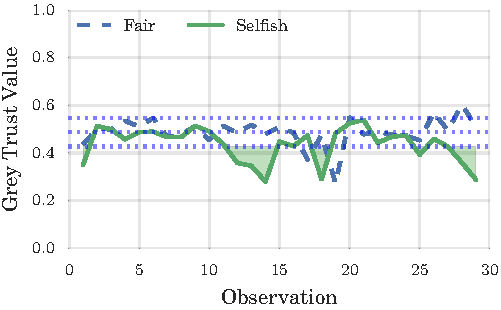
\includegraphics[width=.33\linewidth]{img/trust_bella_all_mobile_emph_ADelay_SelfishTargetSelection} \label{fig:all_mobile_selfish_delay}}
  \subfloat[PLR Emphasised]{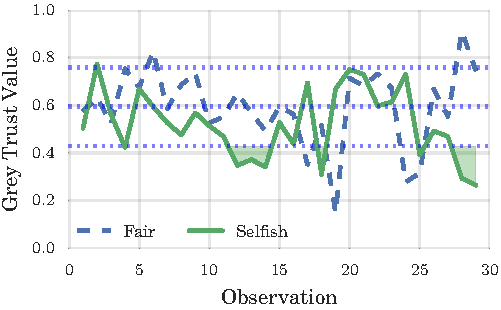
\includegraphics[width=.33\linewidth]{img/trust_bella_all_mobile_emph_PLR_SelfishTargetSelection}\label{fig:all_mobile_selfish_plr}}
  \subfloat[RX Power Emphasised]{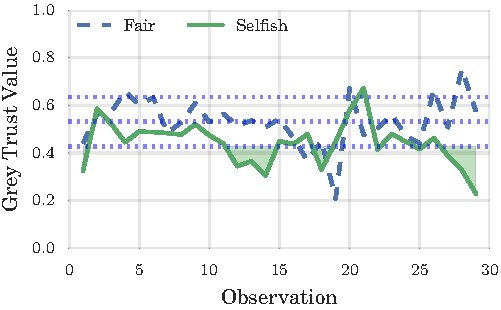
\includegraphics[width=.33\linewidth]{img/trust_bella_all_mobile_emph_ARXP_SelfishTargetSelection} \label{fig:all_mobile_selfish_rxp}}
  \newline
  \subfloat[TX Power Emphasised]{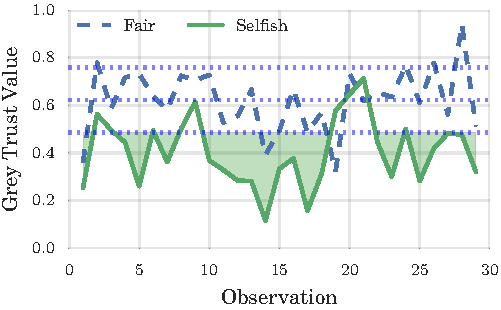
\includegraphics[width=.33\linewidth]{img/trust_bella_all_mobile_emph_ATXP_SelfishTargetSelection}\label{fig:all_mobile_selfish_txp}}
  \subfloat[RX Throughput Emphasised]{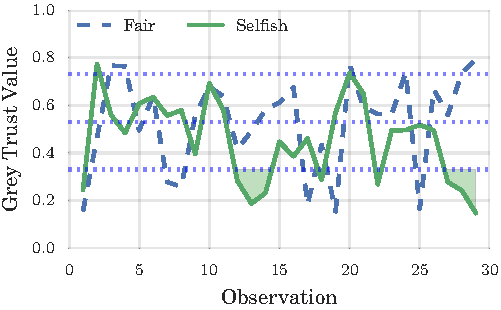
\includegraphics[width=.33\linewidth]{img/trust_bella_all_mobile_emph_RXThroughput_SelfishTargetSelection} \label{fig:all_mobile_selfish_rxthroughput}}
  \subfloat[TX Throughput Emphasised]{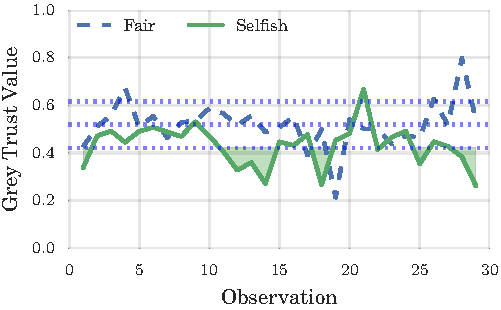
\includegraphics[width=.33\linewidth]{img/trust_bella_all_mobile_emph_TXThroughput_SelfishTargetSelection} \label{fig:all_mobile_selfish_txthroughput}}
\caption{$T_{1,MTFM}$ in the All Mobile case for the Selfish Target Selection behaviour, including dashed $\pm\sigma$ envelope about the fair scenario\hyperlink{fig:selfish_emph_closeup}{\beamergotobutton{Closeup}}}
 
\end{figure}
\end{frame}

\begin{frame}{Metric Weighting}
  Key Observations:
  \begin{itemize}
    \item In MPC case:
      \begin{itemize}
        \item Consistently outside $\pm\sigma$ in most
        \item Particularly PLR
        \item Less so in Delay, $P_{RX}$ and $T_{TX}$
      \end{itemize}
    \item In STS case:
      \begin{itemize}
        \item Less overall impact
        \item Stronger impact of $P_{TX}$
      \end{itemize}
  \end{itemize}

\end{frame}


\subsection{Metric Significance}
\begin{frame}{Regression of Metric Significance}
  Aim: Establish which metrics are important in discriminating behaviours
  \pause
  \begin{itemize}
    \item Distributed Random Forest Regression \autocite{Breiman2001} 
    \item 729 Metric Weight Vectors ($H$), 512 random trees
    \item 16 Random starts of each of the 3 scenarios for 6 nodes for 6 hour ``missions''
    \item Targeting area of $\pm\sigma$ deviation $\int abs(T_m - \overline T_f) - \sigma_{T_f}$
    \item Regression identifies the significance of metrics in classifying between the three possible behaviours
  \end{itemize}

\end{frame}
\begin{frame}{Metric Significance}

  \begin{figure}
    \centering
    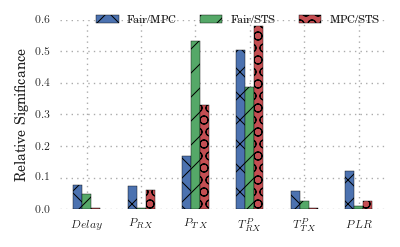
\includegraphics[width=0.95\linewidth]{img/MaliciousSelfishMetricFactors}
    \label{fig:malselfactors}
  \end{figure}
\end{frame}
\begin{frame}{Metric Correlation Combs}
  \begin{table}[h]
    \begin{center}
      \small
      \bgroup
      \def\arraystretch{1.2}%  1 is the default, change whatever you need
      \setlength\tabcolsep{4pt}% 6pt standard
      \begin{tabular}{l|CCCCCC}
        \toprule
        Correlation      & Delay & $P_{RX}$ & $P_{TX}$ & $T^P_{RX}$ & $T^P_{TX}$ & PLR \\
        \midrule
        Fair / MPC       & 0.199 &  0.159   & -0.416  &  0.708   & -0.238   & -0.401\\
        Fair / STS       & 0.179 &  -0.009  &  0.724  & -0.697   & -0.145   & -0.052\\
        MPC / STS        & 0.058 &  -0.134  &  0.146  & -0.768   &  0.052   &  0.146\\
        \bottomrule
      \end{tabular}
      \egroup
    \end{center}
  \end{table}

\end{frame}
\begin{frame}{Key Observations}
  \begin{itemize}
    \item PLR not necessarily the most important metric in \alert{discriminating} behaviours
    \pause\item Combination of Significance and Correlations demonstrate selectivity opportunity
    \pause\item MTFM has capability to finely discriminate between similar misbehaviours
    \pause\item PLR impact is minimal in STS, would not be detected by OTMF/Hermes even in less sparse/harsh environment
    \pause\item Identifying this classification ``comb'' is computationally intensive and grows exponentially with number of metrics involved for brute force regression
  \end{itemize}
\end{frame}


\section*{Summary}

\begin{frame}{Summary}
  % Keep the summary *very short*.
  \begin{itemize}
    \item Trust Underwater is \alert{Hard}, but it's mostly the environments' fault
    \item Single-Metric Trust is \alert{unstable} in such an environment
    \item Multi-Metric Trust works and can \alert{discriminate between behaviours}
    \item \alert{Not all metrics} are equally useful
  \end{itemize}
  
  % The following outlook is optional.
  \pause
  \vskip0pt plus.5fill
  \begin{itemize}
  \item
    Outlook
    \begin{itemize}
    \item Extending to include Physical Metrics
    \item Developing runtime heuristics to improve complexity
    \item Perform untrained classification performance on real data      
    \item Perform / Initiate practical trials in collaborations with NATO CMRE
    \end{itemize}
  \end{itemize}
\end{frame}

\begin{frame}[t,allowframebreaks]
  \frametitle{References}
  \printbibliography[title=References]% [nottype=video]}
\end{frame}

\begin{frame}
  \centerline{Thank You}
\end{frame}

\begin{frame}[allowframebreaks]{Grey Trust Equs}
  \begin{align}
    \label{eq:networkeffects}
    T_{i,j}^{MTFM}=&\frac{1}{2} \cdot \max_s\{f_s(T_{i,j})\} T_{i,j}\\ \notag
    +&\frac{1}{2} \frac{2|N_R| }{2|N_R| + |N_I|}\sum_{n \in N_R} \max_s\{f_s(T_{i,n})\} T_{i,n}\\ \notag
    +&\frac{1}{2} \frac{|N_I| }{2|N_R| + |N_I|}\sum_{n \in N_I} \max_s\{f_s(T_{i,n})\} T_{i,n} 
  \end{align}

  Where $T_{i,n}$ is the subjective trust assessment of $n_i$ by $n_n$, and $f_s = [ f_1,f_2, f_3]$ given as...

  \framebreak

  \begin{align}
    \label{eq:whitenization}
    f_1(x)&= -x+1\notag\\
    f_2(x)&= 
    \begin{cases}
      2x & \text{if }x\leq 0.5\\
      -2x+2 & \text{if }x>0.5
    \end{cases}\\
    f_3(x)&= x\notag
  \end{align}
\hyperlink{fig:node_relationships}{\beamergotobutton{Back}}
\end{frame}

\begin{frame}[allowframebreaks]{Comms Scaling Graphs}

\setcounter{subfigure}{0}% Reset subfigure counter
  \begin{figure}[h]
    \centering
    \subfloat[][All Nodes Static]{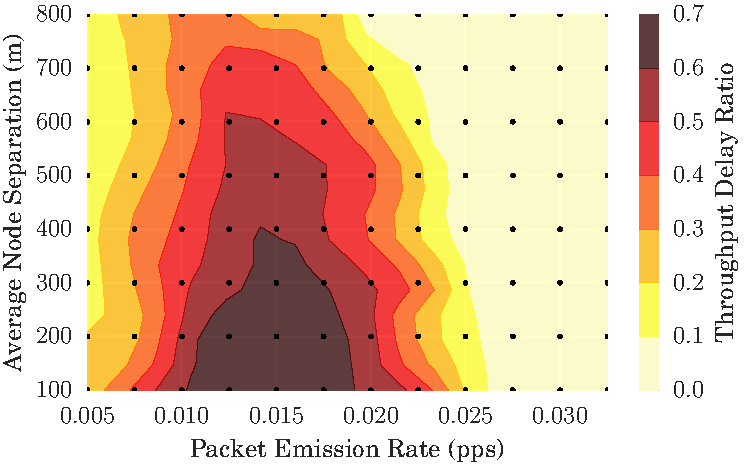
\includegraphics[width=0.35\linewidth]{2d_ratio_static.pdf}}
    \subfloat[][$n_1$ Random Walk]{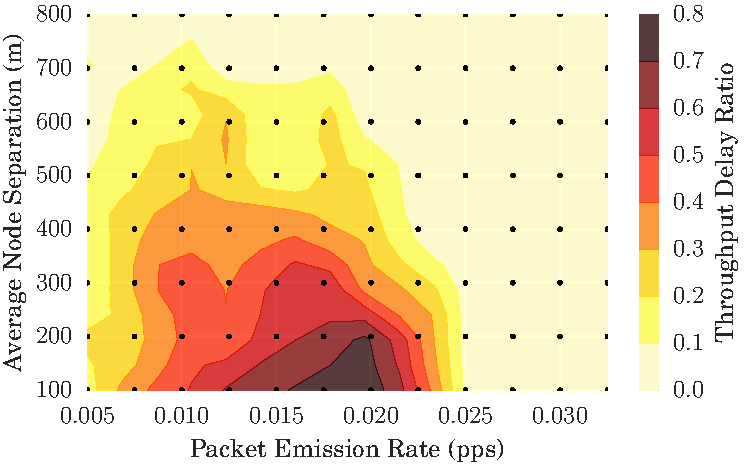
\includegraphics[width=0.35\linewidth]{2d_ratio_single_mobile.pdf}}\\
    \subfloat[][All nodes but $n_1$ Random Walk]{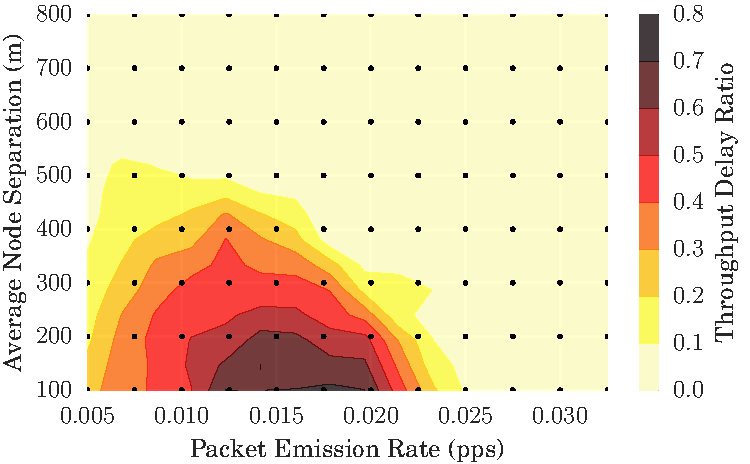
\includegraphics[width=0.35\linewidth]{2d_ratio_allbut1.pdf}}
    \subfloat[][All nodes Random Walk]{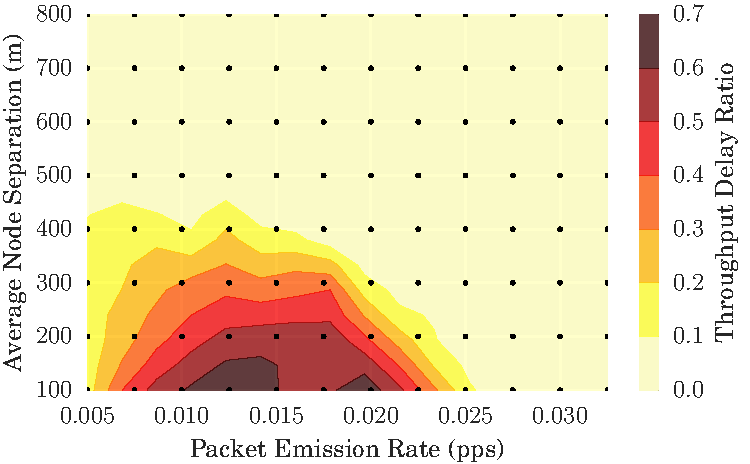
\includegraphics[width=0.35\linewidth]{2d_ratio_all_mobile.pdf}}
    \label{fig:CommsThroughputRatios}
  \end{figure}
\hyperlink{scaling}{\beamergotobutton{Back}}

\end{frame}

\begin{frame}[shrink]{System Model Constraints}
\centering
\begin{table}[h]
  \caption{Comparison of system model constraints as applied between Terrestrial and Marine communications
  \hyperlink{scaling}{\beamergotobutton{Back}}
  } \label{tab:sysconstraints}
  \begin{center}
    \setlength{\tabcolsep}{8pt}
    \begin{tabular}{lccc}
      \toprule
      Parameter & Unit & Terrestrial & Marine \\
      \midrule
      Simulated Duration & $s$ & 300 & 18000\\
      Trust Sampling Period & $s$ & 1 & 600 \\
      Simulated Area & $km^2$ & 0.7 & 0.7-4 \\
      Transmission Range & $km$ & 0.25 & 1.5 \\
      Physical Layer & & RF(802.11) & Acoustic\\
      Propagation Speed& $m/s$ & $3\times10^8$ & 1490\\
      Center Frequency& $Hz$ & $2.6\times10^9$ & $2 \times 10^4$ \\
      Bandwidth& $Hz$ & $22\times10^6$ & $1\times10^4$\\
      MAC Type & & CSMA/DCF & CSMA/CA\\
      Routing Protocol & & DSDV & FBR \\
      Max Speed & $ms^{-1}$ & 5 & 1.5 \\
      Max Data Rate & $bps$ & $5\times10^6$ & $\approx 240$ \\
      Packet Size & bits & 4096 &  9600 \\
      Single Transmission Duration & $s$ & 10 & 32 \\
      Single Transmission Size & bits & $10^7$ & $9600$ \\
      \bottomrule
    \end{tabular}
    \setlength{\tabcolsep}{6pt}
  \end{center}
\end{table}

\end{frame}

\begin{frame}{MTFM Operation Detail}
%
\setcounter{subfigure}{0}% Reset subfigure counter
\label{fig:trust_mobility_closeup}%
\begin{figure}[h]
  \subfloat[Fair Static]{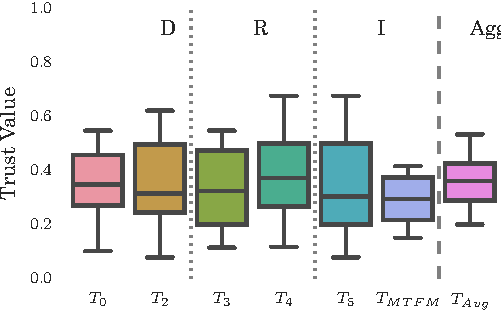
\includegraphics[width=1.0\linewidth]{trust_bella_static_fair} \label{fig:trust_static}}
\end{figure}
  \hyperlink{fig:trust_mobility}{\beamergotobutton{Back}}
\end{frame}
\begin{frame}{MTFM Operation Detail}
\begin{figure}[h]
  \subfloat[Malicious Static]{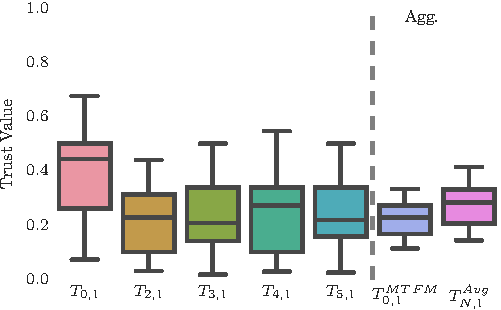
\includegraphics[width=1.0\linewidth]{trust_bella_static_malicious} \label{fig:trust_static_mal}}
\end{figure}
  \hyperlink{fig:trust_mobility}{\beamergotobutton{Back}}
\end{frame}
\begin{frame}{MTFM Operation Detail}
\begin{figure}[h]
  \subfloat[Selfish Static]{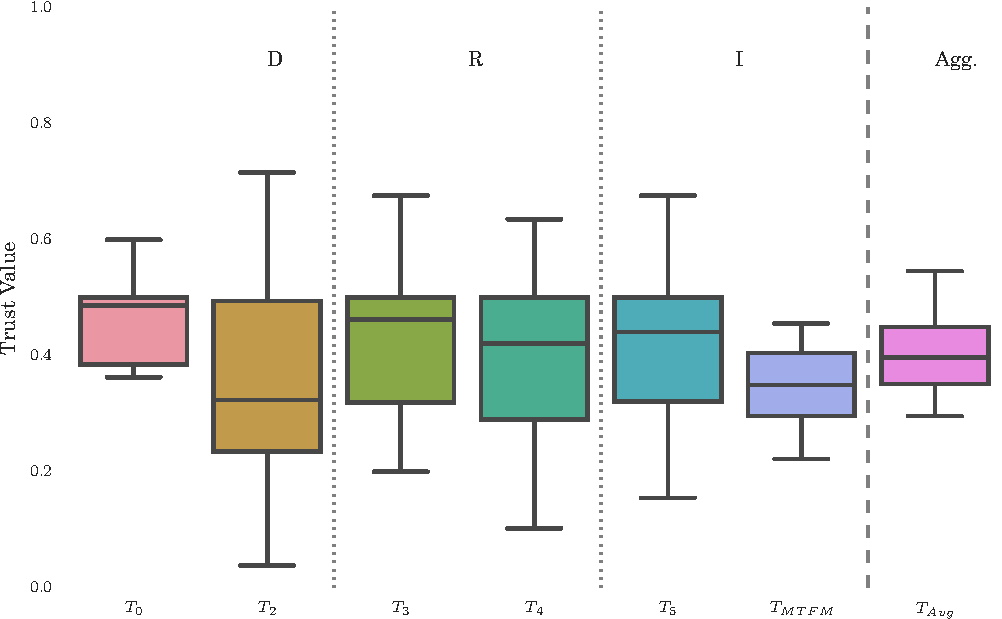
\includegraphics[width=1.0\linewidth]{trust_bella_static_selfish} \label{fig:trust_static_sel}}
\end{figure}
  \hyperlink{fig:trust_mobility}{\beamergotobutton{Back}}
\end{frame}
\begin{frame}{MTFM Operation Detail}
\begin{figure}[h]
  \subfloat[Fair Mobile]{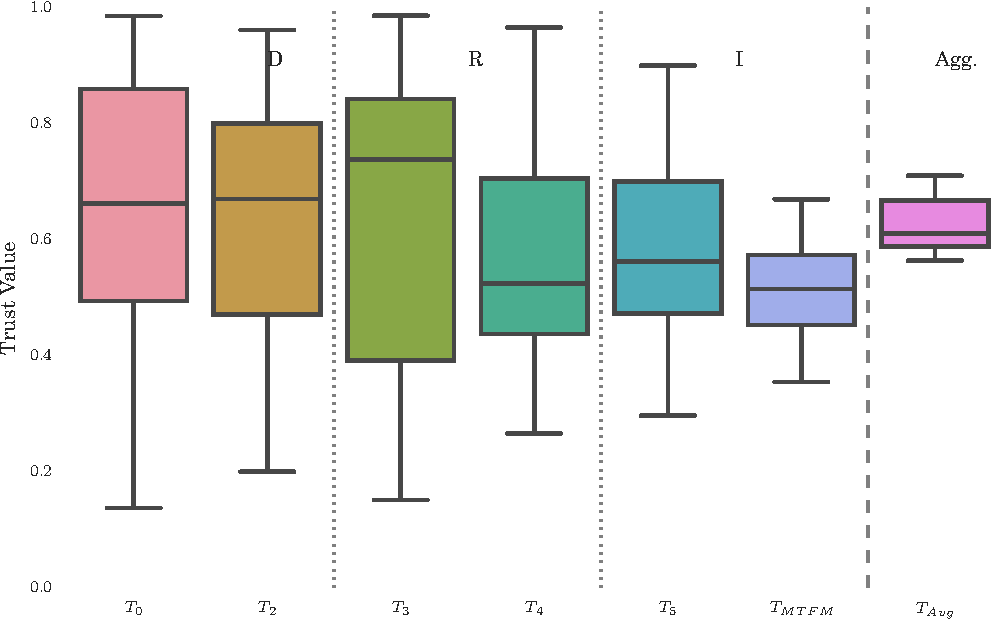
\includegraphics[width=1.0\linewidth]{trust_bella_all_mobile_fair}  \label{fig:trust_all_mobile}}
\end{figure}
  \hyperlink{fig:trust_mobility}{\beamergotobutton{Back}}
\end{frame}
\begin{frame}{MTFM Operation Detail}
\begin{figure}[h]
  \subfloat[Malicious Mobile]{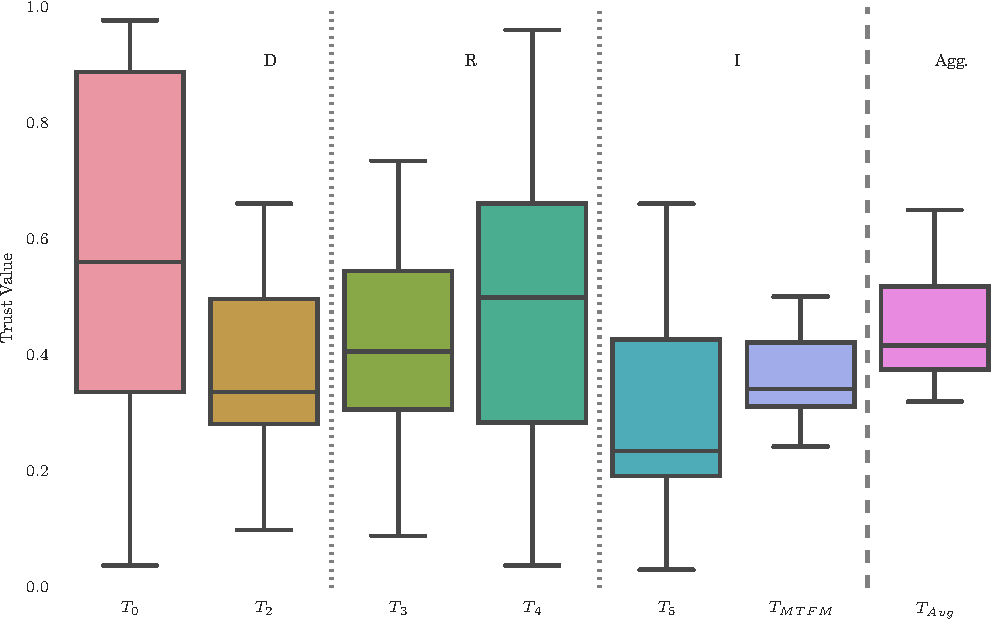
\includegraphics[width=1.0\linewidth]{trust_bella_all_mobile_malicious}  \label{fig:trust_all_mobile_mal}}
\end{figure}
  \hyperlink{fig:trust_mobility}{\beamergotobutton{Back}}
\end{frame}
\begin{frame}{MTFM Operation Detail}
\begin{figure}[h]
  \subfloat[Selfish Mobile]{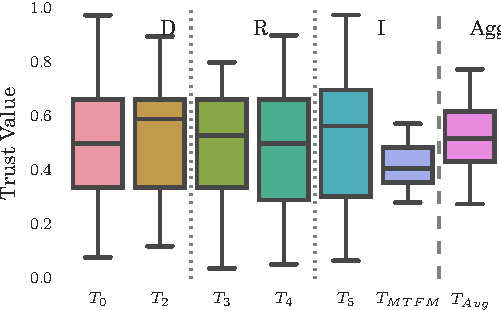
\includegraphics[width=1.0\linewidth]{trust_bella_all_mobile_selfish}  \label{fig:trust_all_mobile_sel}}

\end{figure}
  \hyperlink{fig:trust_mobility}{\beamergotobutton{Back}}
\end{frame}


\begin{frame}{MTFM Malicious Power Control Detail}
\setcounter{subfigure}{0}% Reset subfigure counter
\label{fig:badmouth_emph_closeup}%
\begin{figure}[h]
  \subfloat[Delay Emphasised]{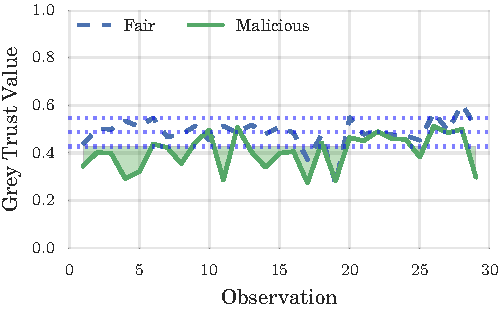
\includegraphics[width=\linewidth]{img/trust_bella_all_mobile_emph_ADelay_BadMouthingPowerControl} \label{fig:all_mobile_badmouthing_delay}}
\end{figure}
  \hyperlink{fig:all_mobile_badmouthing}{\beamergotobutton{Back}}
\end{frame}
\begin{frame}{MTFM Malicious Power Control Detail}
\begin{figure}[h]
  \subfloat[PLR Emphasised]{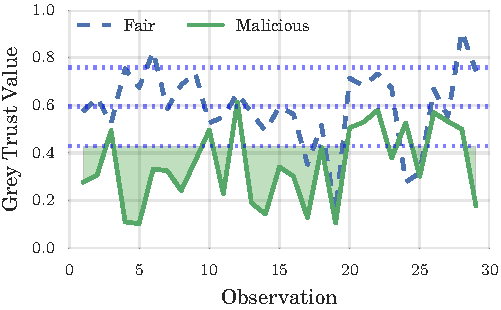
\includegraphics[width=\linewidth]{img/trust_bella_all_mobile_emph_PLR_BadMouthingPowerControl}\label{fig:all_mobile_badmouthing_plr}}
\end{figure}
  \hyperlink{fig:all_mobile_badmouthing}{\beamergotobutton{Back}}
\end{frame}
\begin{frame}{MTFM Malicious Power Control Detail}
\begin{figure}[h]
  \subfloat[RX Power Emphasised]{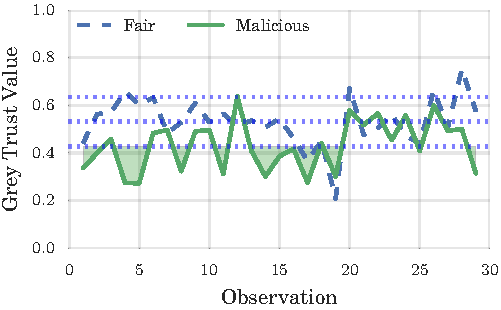
\includegraphics[width=\linewidth]{img/trust_bella_all_mobile_emph_ARXP_BadMouthingPowerControl} \label{fig:all_mobile_badmouthing_rxp}}
\end{figure}
  \hyperlink{fig:all_mobile_badmouthing}{\beamergotobutton{Back}}
\end{frame}
\begin{frame}{MTFM Malicious Power Control Detail}
\begin{figure}[h]
  \subfloat[TX Power Emphasised]{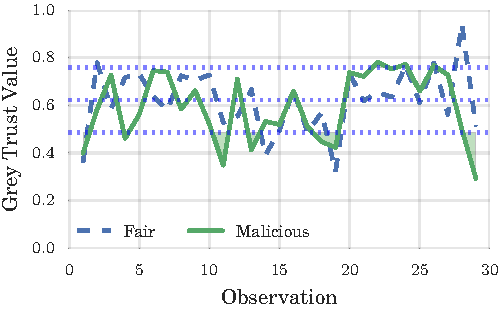
\includegraphics[width=\linewidth]{img/trust_bella_all_mobile_emph_ATXP_BadMouthingPowerControl}\label{fig:all_mobile_badmouthing_txp}}
\end{figure}
  \hyperlink{fig:all_mobile_badmouthing}{\beamergotobutton{Back}}
\end{frame}
\begin{frame}{MTFM Malicious Power Control Detail}
\begin{figure}[h]
  \subfloat[RX Throughput Emphasised]{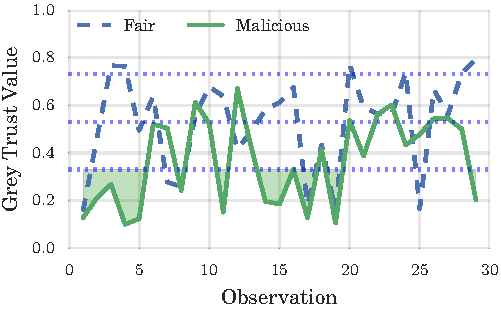
\includegraphics[width=\linewidth]{img/trust_bella_all_mobile_emph_RXThroughput_BadMouthingPowerControl} \label{fig:all_mobile_badmouthing_rxthroughput}}
\end{figure}
  \hyperlink{fig:all_mobile_badmouthing}{\beamergotobutton{Back}}
\end{frame}
\begin{frame}{MTFM Malicious Power Control Detail}
\begin{figure}[h]
  \subfloat[TX Throughput Emphasised]{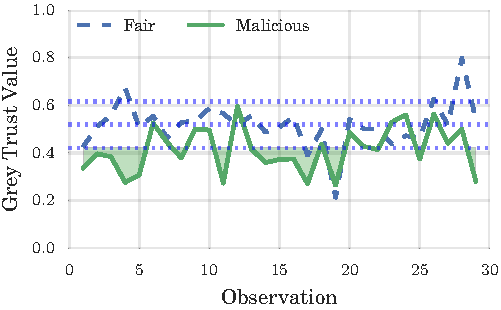
\includegraphics[width=\linewidth]{img/trust_bella_all_mobile_emph_TXThroughput_BadMouthingPowerControl} \label{fig:all_mobile_badmouthing_txthroughput}}
\end{figure}
  \hyperlink{fig:all_mobile_badmouthing}{\beamergotobutton{Back}}
\end{frame}
\begin{frame}{MTFM Selfish Target Selection Detail}
\setcounter{subfigure}{0}% Reset subfigure counter
\label{fig:selfish_emph_closeup}%
\begin{figure}[h]
  \subfloat[Delay Emphasised]{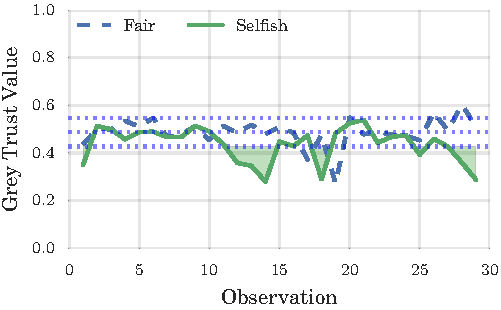
\includegraphics[width=\linewidth]{img/trust_bella_all_mobile_emph_ADelay_SelfishTargetSelection} \label{fig:all_mobile_selfish_delay}}
\end{figure}
  \hyperlink{fig:all_mobile_selfish}{\beamergotobutton{Back}}
\end{frame}
\begin{frame}{MTFM Selfish Target Selection Detail}
\begin{figure}[h]
  \subfloat[PLR Emphasised]{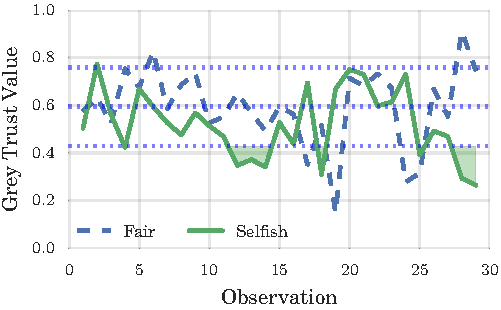
\includegraphics[width=\linewidth]{img/trust_bella_all_mobile_emph_PLR_SelfishTargetSelection}\label{fig:all_mobile_selfish_plr}}
\end{figure}
  \hyperlink{fig:all_mobile_selfish}{\beamergotobutton{Back}}
\end{frame}
\begin{frame}{MTFM Selfish Target Selection Detail}
\begin{figure}[h]
  \subfloat[RX Power Emphasised]{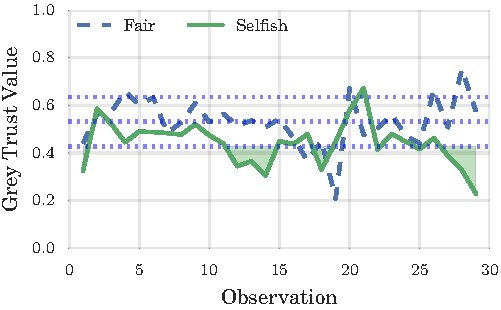
\includegraphics[width=\linewidth]{img/trust_bella_all_mobile_emph_ARXP_SelfishTargetSelection} \label{fig:all_mobile_selfish_rxp}}
\end{figure}
  \hyperlink{fig:all_mobile_selfish}{\beamergotobutton{Back}}
\end{frame}
\begin{frame}{MTFM Selfish Target Selection Detail}
\begin{figure}[h]
  \subfloat[TX Power Emphasised]{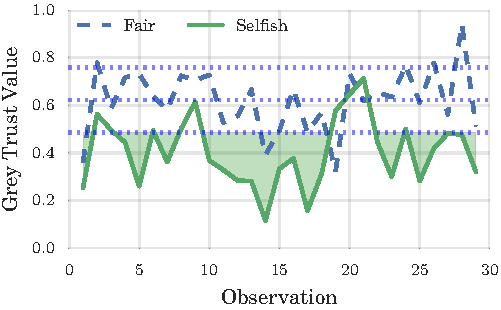
\includegraphics[width=\linewidth]{img/trust_bella_all_mobile_emph_ATXP_SelfishTargetSelection}\label{fig:all_mobile_selfish_txp}}
\end{figure}
  \hyperlink{fig:all_mobile_selfish}{\beamergotobutton{Back}}
\end{frame}
\begin{frame}{MTFM Selfish Target Selection Detail}
\begin{figure}[h]
  \subfloat[RX Throughput Emphasised]{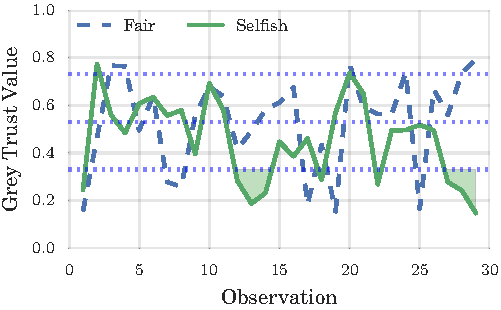
\includegraphics[width=\linewidth]{img/trust_bella_all_mobile_emph_RXThroughput_SelfishTargetSelection} \label{fig:all_mobile_selfish_rxthroughput}}
\end{figure}
  \hyperlink{fig:all_mobile_selfish}{\beamergotobutton{Back}}
\end{frame}
\begin{frame}{MTFM Selfish Target Selection Detail}
\begin{figure}[h]
  \subfloat[TX Throughput Emphasised]{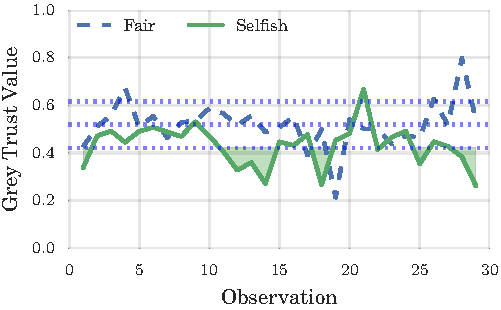
\includegraphics[width=\linewidth]{img/trust_bella_all_mobile_emph_TXThroughput_SelfishTargetSelection} \label{fig:all_mobile_selfish_txthroughput}}
\end{figure}
  \hyperlink{fig:all_mobile_selfish}{\beamergotobutton{Back}}
\end{frame}

\end{document}
